%!TEX root = ../thesis.tex
% ******************************* Thesis Appendix F*******************************

\chapter{Analysis Chains}

\begin{figure}[!h]
 \centering
 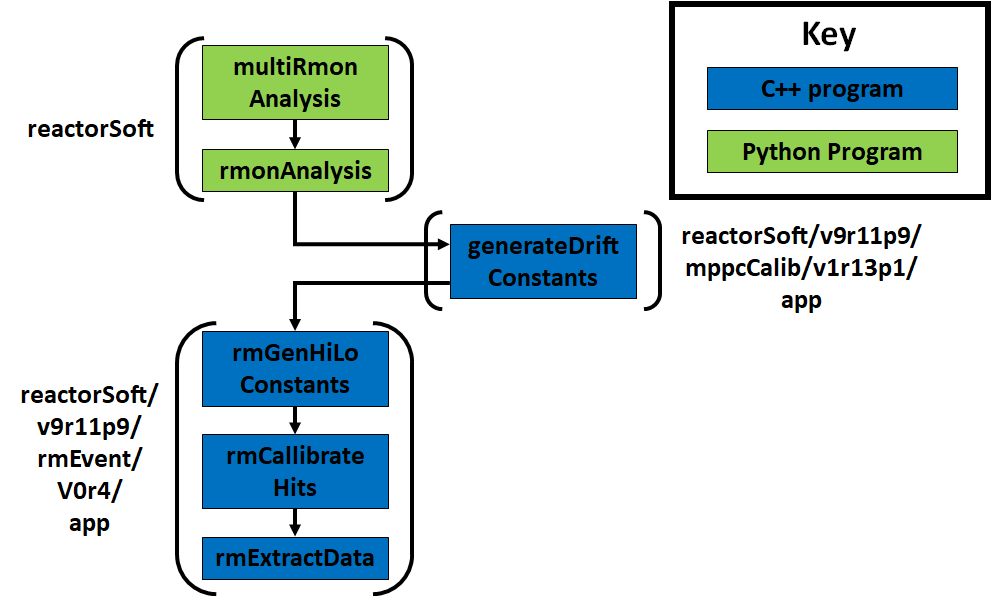
\includegraphics[width=\linewidth]{Chapter5/Figs/Raster/mattMurdocksChain.png}
 \captionof{figure}[The analysis chain for the original detector's \texttt{.mid.gz} files.]{The analysis chain for the original detector's \texttt{.mid.gz} files. The python programs are wrappers that control the setup of the software, which programs C++ to run, and the number of instances to run. The C++ programs generate the information needed for calibration and then extract the information to .root files. This is only a small fraction of the analysis chain.} 
 \label{fig:mattMurdocksChain}
\end{figure}
 
\begin{figure}[!h]
 \centering
 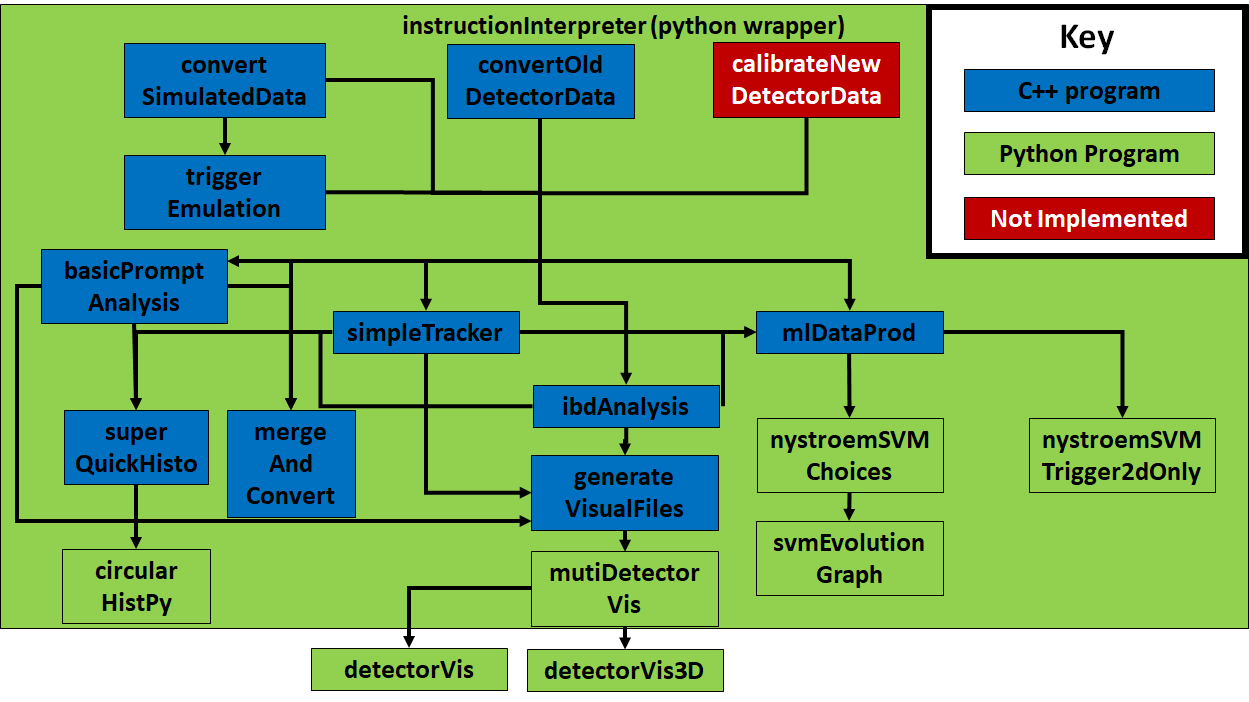
\includegraphics[width=\linewidth]{Chapter5/Figs/Raster/analysisChainRevisedAgain.png}
 \captionof{figure}[The analysis chain for analysing detailed event information.]{The analysis chain for the detector. It is able to process both simulated and measured data. It uses a combination of python programs to handle visualisation and machine learning and C++ programs to process the data. The python program \texttt{instructionInterpreter} that functions as a wrapper allows for the creation of macro files so results are highly replicable. The C++ programs are multi-threaded. The python programs are in the \texttt{repository} the C++ programs are in \texttt{repository/prg}.} 
 \label{fig:analysisChain}
\end{figure}